\documentclass{beamer}


% Beamer settings
\usecolortheme{rose}
\beamertemplatenavigationsymbolsempty
\setbeamertemplate{footline}[frame number]

\titlegraphic{%

\includegraphics[height=1cm]{logo-full-colour.png}}

\addtobeamertemplate{frametitle}{}{%
\begin{tikzpicture}[remember picture,overlay]
\node[anchor=north east,yshift=2pt] at (current page.north east) {
\includegraphics[height=1cm]{logo-full-colour.png}};
\end{tikzpicture}}

% Packages
\usepackage{amsmath}

\usepackage{tikz}
\usetikzlibrary{positioning}
\usetikzlibrary{fit}

\usepackage{pgfplots}
\usepgfplotslibrary{fillbetween}

\usepackage{minted}
\usepackage[T1]{fontenc} % Required by minted to ensure dollar signs are produced instead of pound (sterling) signs

\usepackage{multicol}

\usepackage{booktabs}

\usepackage{adjustbox}

% Author
\author{Simon McIntosh-Smith \& Tom Deakin\\University of Bristol}

\date{}



\title{OpenMP for Computational Scientists}
\subtitle{3: Vectoristation and optimisations}

\begin{document}

\frame{\titlepage}

%-------------------------------------------------------------------------------
\begin{frame}
\frametitle{Outline}
Now you know how to parallelise programs using OpenMP, how do you write fast programs in OpenMP?
\begin{itemize}
  \item The cache hierarchy
  \item Performance analysis
  \item Vectorisation
  \item Array of structures vs Structure of arrays
  \item Memory access patterns
  \item Memory alignment
\end{itemize}
\end{frame}

%-------------------------------------------------------------------------------
\section{The cache hierarchy}
\begin{frame}
\frametitle{Cache hierarchy}
\end{frame}

%-------------------------------------------------------------------------------
\section{Performance analysis}
\begin{frame}
\frametitle{Roofline models}
\end{frame}

%-------------------------------------------------------------------------------
\section{Vectorisation}
\begin{frame}
\frametitle{Vectorisation}
$$C=A+B$$
\begin{columns}
\begin{column}{0.5\textwidth}
Scalar operations \\
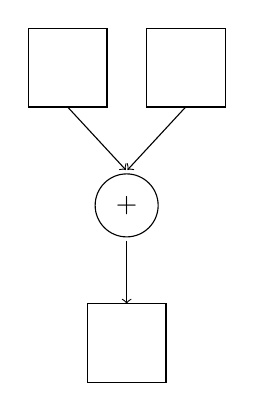
\begin{tikzpicture}
  \draw (-0.5,2) rectangle (0.5,3);
  \draw (1,2) rectangle (2,3);
  \draw[->] (0,2) -- (.74,1.2);
  \draw[->] (1.5,2) -- (.76,1.2);
  \draw (.75,.75) circle (.4cm);
  \draw (.75,.75) node {$+$};
  \draw[->] (.75,0.3) -- (.75,-0.5);
  \draw (.25,-1.5) rectangle (1.25,-0.5);
\end{tikzpicture}
\end{column}

\begin{column}{0.5\textwidth}
Vector operations \\
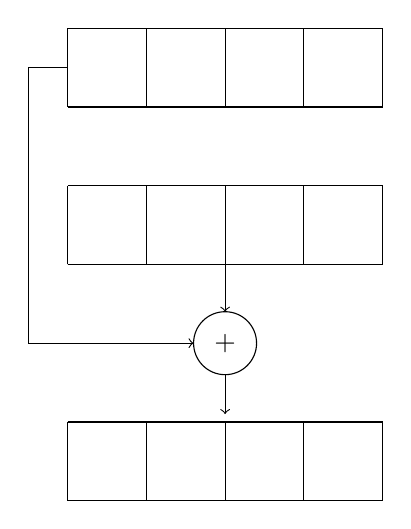
\begin{tikzpicture}
  \draw[step=1cm] (0,2) grid (4,3);
  \draw[step=1cm] (0,0) grid (4,1);
  \draw[->] (2,0) -- (2,-0.6);
  \draw[->] (0,2.5) -- (-0.5,2.5) -- (-0.5,-1) -- (1.6,-1);
  \draw (2,-1) circle (.4cm);
  \draw (2,-1) node {$+$};
  \draw[->] (2,-1.4) -- (2,-1.9);
  \draw[step=1cm] (0,-3) grid (4,-2);
\end{tikzpicture}
\end{column}
\end{columns}

\end{frame}

%-------------------------------------------------------------------------------
\begin{frame}
\frametitle{Why vectorise?}
\begin{itemize}
  \item Vectorisation gives you more compute per cycle.
  \item Hence increases the FLOPS/s rate of the processor.
  \item Also results in fewer instructions to process (less presure on instruction decode units).
  \item Vectors help make good use of the memory hierarchy.
  \item Helps you write code which has good access patterns to maximise bandwidth.
\end{itemize}
\end{frame}

%-------------------------------------------------------------------------------
\begin{frame}
\frametitle{Auto-vectorisation}
\begin{itemize}
  \item Modern compilers are very good to automatically vectorising your loops.
  \item Fortran helps as arrays do not alisas (overlap).
  \item But compiler needs to be sure it's safe to vectorise.
  \item Read compiler reports to see if it's already vectorising.
    \begin{itemize}
      \item Intel: \mintinline{bash}|-qopt-report=5|
      \item Cray: \mintinline{bash}|-hlist=a|
    \end{itemize}
  \item Often memory access pattern which prevents (efficient) auto-vectorisation.
\end{itemize}
\end{frame}

%-------------------------------------------------------------------------------
\subsection{OpenMP SIMD}
\begin{frame}[fragile]
\frametitle{OpenMP SIMD}
\begin{itemize}
  \item Sometimes the compiler needs help in confirming loops are vectorisable.
  \item OpenMP \mintinline{fortran}|simd| constructs give this information.
  \item Can combine with \mintinline{fortran}|parallel do| construct to ensure a parallel vector loop.
  \item Generally want to vectorise inner loops and parallelise outer loops.
\end{itemize}

\begin{minted}[frame=single]{fortran}
!$omp simd
do i = 1, N
  C(i) = A(i)+B(i)
end do
!$omp end simd
\end{minted}
\end{frame}

%-------------------------------------------------------------------------------
\begin{frame}[fragile]
\frametitle{SIMD functions}
Often have written an update function to update values in the loop:
\begin{minted}[frame=single]{fortran}
do i = 1, N
  A(i) = magic_maths(A(i))
end do
\end{minted}

\begin{itemize}
  \item The situation gets complicated.
  \item If the function is small, then likely inlined and loop will auto-vectorise.
  \item Otherwise need to use the \mintinline{fortran}|simd| construct, but need compiler to create a vector version of the function.
\end{itemize}

\begin{minted}[frame=single]{fortran}
function magic_maths(value) result(r)
!$omp declare simd(magic_maths)
  implicit none
  real(kind=8) :: value, r
  r = value * value
end function
\end{minted}

\end{frame}

%-------------------------------------------------------------------------------
\begin{frame}[fragile]
\frametitle{SIMD clauses}
\begin{itemize}
  \item All the usual data-sharing and reduction clauses can be applied.
  \item \mintinline{fortran}|safelen(4)|: distance between iterations where its safe to vectorise.
  \begin{minted}[frame=single]{fortran}
  !$omp simd safelen(4)
  do i = 1, N-4
    A(i) = A(i) + A(i+4)
  end do
  !$omp end simd
  \end{minted}
  \item \mintinline{fortran}|simdlen(4)|: prefered iterations to be performed concurrently as a vector.
\end{itemize}
\end{frame}

%-------------------------------------------------------------------------------
\begin{frame}[fragile]
\frametitle{SIMD clauses}
\begin{itemize}
  \item \mintinline{fortran}|linear(var)|: variable is private and linear to the loop iterator.
  \begin{minted}[frame=single]{fortran}
  !$omp simd linear(j)
  do i = 1, N
    j = j + 1
    A(j) = B(i)
  end do
  !$omp end simd
  \end{minted}
  \item \mintinline{fortran}|aligned(var)|: says the array is aligned (more on this shortly).
  \item \mintinline{fortran}|uniform(var)|: for \mintinline{fortran}|declare simd| construct, the variable is the same in all vector lanes.
\end{itemize}
\end{frame}

%-------------------------------------------------------------------------------
\section{Derived types}
\begin{frame}[fragile]
\frametitle{Derived types}
2D grid of cells; each cell containing 4 different values.
\begin{minted}[frame=single,linenos,fontsize=\small]{fortran}
type cell
  real(kind=8) :: property1
  real(kind=8) :: property2
  real(kind=8) :: property3
  real(kind=8) :: property4
end type

type(cell), allocatable :: grid(:,:)

do j = 1, ny
  do i = 1, nx
    grid(i,j)%property1 = update_1()
    grid(i,j)%property2 = update_2()
    grid(i,j)%property3 = update_3()
    grid(i,j)%property4 = update_4()
  end do
end do
\end{minted}
\end{frame}

%-------------------------------------------------------------------------------
\begin{frame}
\frametitle{Derived types}
\begin{itemize}
  \item What do Fortran derived types look like in memory?
  \item Organised as an array of structures.
  \item<2-> What happens when we vectorise?
\end{itemize}

\begin{adjustbox}{max width={\textwidth}}
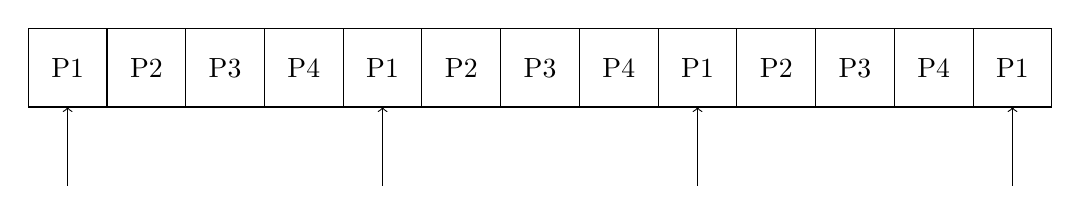
\begin{tikzpicture}
  \draw[step=1cm] (0,0) grid (13,1);
  \foreach \i in {0,4,8,12} {
    \draw (\i+.5,.5) node {P1};
  }
  \foreach \i in {0,4,8} {
    \draw (\i+1.5,.5) node {P2};
    \draw (\i+2.5,.5) node {P3};
    \draw (\i+3.5,.5) node {P4};
  }

  \pause
  \foreach \i in {0,4,8,12} {
    \draw[->] (\i+.5,-1) -- (\i+.5,0);
  }
\end{tikzpicture}
\end{adjustbox}

\pause
\begin{itemize}
  \item The \mintinline{fortran}|property1| values are gathered into a vector register.
  \item After the computation, the results are scattered back into memory.
  \item A cache line is 64 bytes, so only the first two values are on the first cache line.
  \item Must read two cache lines to fill the vector up.
\end{itemize}
\end{frame}

%-------------------------------------------------------------------------------
\begin{frame}[fragile]
\frametitle{Structure of arrays}
Switch type around to have an array per property.
\begin{minted}[frame=single,linenos]{fortran}
type grid
  real(kind=8), allocatable :: property1(:,:)
  real(kind=8), allocatable :: property2(:,:)
  real(kind=8), allocatable :: property3(:,:)
  real(kind=8), allocatable :: property4(:,:)
end type

do j = 1, ny
  do i = 1, nx
    grid%property1(i,j) = update_1()
    grid%property2(i,j) = update_2()
    grid%property3(i,j) = update_3()
    grid%property4(i,j) = update_4()
  end do
end do
\end{minted}
\end{frame}

%-------------------------------------------------------------------------------
\begin{frame}
\frametitle{Structure of arrays}
\begin{itemize}
  \item What happens when we vectorise?
\end{itemize}

\begin{adjustbox}{max width={\textwidth}}
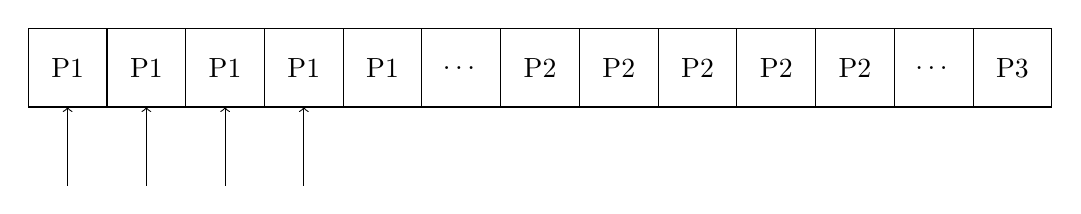
\begin{tikzpicture}
  \draw[step=1cm] (0,0) grid (13,1);
  \foreach \i in {0,...,4} {
    \draw (\i+.5,.5) node {P1};
  }
  \draw (5.5,.5) node {\dots};

  \foreach \i in {5,...,9} {
    \draw (\i+1.5,.5) node {P2};
  }
  \draw (11.5,.5) node {\dots};

  \foreach \i in {10} {
    \draw (\i+2.5,.5) node {P3};
  }

  \pause
  \foreach \i in {0,...,3} {
    \draw[->] (\i+.5,-1) -- (\i+.5,0);
  }
\end{tikzpicture}
\end{adjustbox}

\pause
\begin{itemize}
  \item Coalesced memory accesses are key for high performance code.
  \item Adjacent vector lanes read adjacent memory locations.
  \item A cache line is 64 bytes, so can fill the vector from a single cache line.
  \item More efficient vectorisation.
\end{itemize}
\end{frame}

%-------------------------------------------------------------------------------
\section{Memory access patterns}
\begin{frame}[fragile]
\frametitle{Memory access patterns}
\begin{minted}{fortran}
do i = 1, N
  val = A(i)
end do
\end{minted}
\begin{adjustbox}{max width={\textwidth}}
\begin{tikzpicture}
  \draw[step=1cm] (-3,0) grid (11,1);
  \draw[dashed] (0,-.5) -- (0,1.5);
  \draw[dashed] (8,-.5) -- (8,1.5);
  \draw (0,-1) node {64 byte boundary};
  \foreach \i in {0,...,7} {
    \draw[->] (\i+.5,2) -- (\i+.5,1.2);
  }
\end{tikzpicture}
\end{adjustbox}
\begin{itemize}
  \item Ideal memory access pattern.
  \item All access is coalesced.
  \item Vectors are aligned to cache line boundary.
\end{itemize}
\end{frame}

%-------------------------------------------------------------------------------
\begin{frame}[fragile]
\frametitle{Memory access patterns}
\begin{minted}{fortran}
do i = 1, N
  val = A(i+3)
end do
\end{minted}
\begin{adjustbox}{max width={\textwidth}}
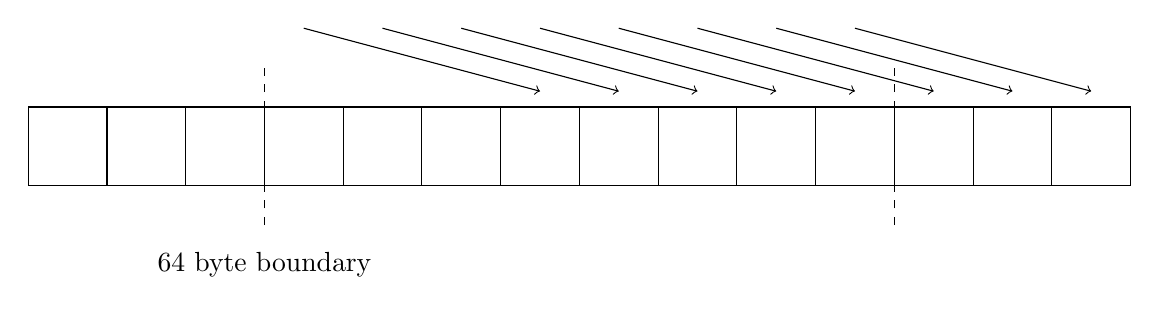
\begin{tikzpicture}
  \draw[step=1cm] (-3,0) grid (11,1);
  \draw[dashed] (0,-.5) -- (0,1.5);
  \draw[dashed] (8,-.5) -- (8,1.5);
  \draw (0,-1) node {64 byte boundary};
  \foreach \i in {0,...,7} {
    \draw[->] (\i+.5,2) -- (3+\i+.5,1.2);
  }
\end{tikzpicture}
\end{adjustbox}
\begin{itemize}
  \item OK memory access pattern.
  \item All access is coalesced, but split across cache line.
  \item Still get good use of cache lines, but not as efficient as aligned version.
\end{itemize}
\end{frame}

%-------------------------------------------------------------------------------
\begin{frame}[fragile]
\frametitle{Memory access patterns}
\begin{minted}{fortran}
do i = 1, N
  val = A(j,i) % A(j+3*i)
end do
\end{minted}
\begin{adjustbox}{max width={\textwidth}}
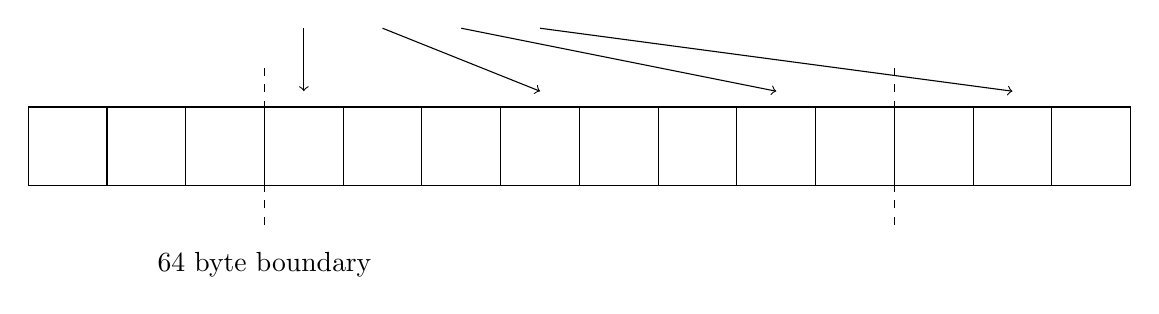
\begin{tikzpicture}
  \draw[step=1cm] (-3,0) grid (11,1);
  \draw[dashed] (0,-.5) -- (0,1.5);
  \draw[dashed] (8,-.5) -- (8,1.5);
  \draw (0,-1) node {64 byte boundary};
  \foreach \i in {0,...,3} {
    \draw[->] (\i+.5,2) -- (3*\i+.5,1.2);
  }
\end{tikzpicture}
\end{adjustbox}
\begin{itemize}
  \item Strided access results in multiple memory transactions.
  \item Kills throughput due to poor reuse of cached data.
  \item Very easy to fall into this trap with multi-dimensional arrays.
  \item Check your strides!
\end{itemize}
\end{frame}

%-------------------------------------------------------------------------------
\begin{frame}[fragile]
\frametitle{Memory access patterns}
\begin{minted}{fortran}
do i = 1, N
  val = A(B(i))
end do
\end{minted}
\begin{adjustbox}{max width={\textwidth}}
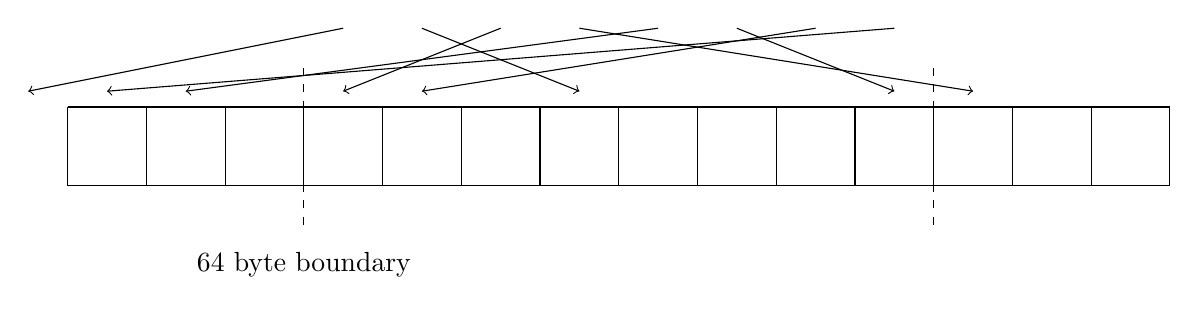
\begin{tikzpicture}
  \draw[step=1cm] (-3,0) grid (11,1);
  \draw[dashed] (0,-.5) -- (0,1.5);
  \draw[dashed] (8,-.5) -- (8,1.5);
  \draw (0,-1) node {64 byte boundary};
  \draw[->] (0.5,2) -- (-3.5,1.2);
  \draw[->] (1.5,2) -- (3.5,1.2);
  \draw[->] (2.5,2) -- (0.5,1.2);
  \draw[->] (3.5,2) -- (8.5,1.2);
  \draw[->] (4.5,2) -- (-1.5,1.2);
  \draw[->] (5.5,2) -- (7.5,1.2);
  \draw[->] (6.5,2) -- (1.5,1.2);
  \draw[->] (7.5,2) -- (-2.5,1.2);
\end{tikzpicture}
\end{adjustbox}
\begin{itemize}
  \item Essentially random access to memory.
  \item Little reuse of cache lines.
  \item Unpredictable pattern, so hardware prefetchers won't work efficiently.
  \item Very challenging!
\end{itemize}
\end{frame}

%-------------------------------------------------------------------------------
\section{Alignment}
\begin{frame}
\frametitle{Alignment}
\begin{itemize}
  \item If we can align arrays, we get better vectorisation; specifically load/stores are faster.
  \item Taking advantage of alignment is a two stage process:
    \begin{enumerate}
      \item Align the memory on allocation.
      \item Tell the compiler the access is aligned.
    \end{enumerate}
  \item Aligned allocations are (currently) unfortunately vendor specific.
  \item OpenMP can help with telling the compiler the data is aligned.
  \item Future OpenMP should have aligned allocators.
\end{itemize}
TODO: Issues with 2D
\end{frame}

%-------------------------------------------------------------------------------
\begin{frame}[fragile]
\frametitle{Aligning allocations}
Generally focus on the Intel compiler.
\begin{itemize}
  \item Align all allocations of arrays (not in derived types) with compiler flag: \mintinline{bash}|-align array64byte|
  \item Use an Intel compiler directive on array definition:
  \begin{minted}[frame=single]{fortran}
  real(kind=8), allocatable :: A(:,:)
  !dir$ attributes align:64 :: A
  \end{minted}
  \item Allocate memory in C, and convert to Fortran \mintinline{fortran}|pointer|:
  \begin{minted}[frame=single,breaklines]{c}
  double * alloc(int *len) {
    return (double *)aligned_alloc(64, sizeof(double)*(*len));
  }
  \end{minted}
  \begin{minted}[frame=single]{fortran}
  real(kind=8), pointer :: A(:,:)
  type(c_ptr) :: A_ptr
  A_ptr = alloc(nx*ny)
  call c_f_pointer(A_ptr, A, (/ nx, ny/))
  \end{minted}
\end{itemize}
\end{frame}

%-------------------------------------------------------------------------------
\begin{frame}[fragile]
\frametitle{Telling the compiler about alignment}
\begin{itemize}
  \item Use OpenMP \mintinline{fortran}|simd aligned| clause:
  \begin{minted}[frame=single,fontsize=\small]{fortran}
  !$omp simd aligned(A:64)
  do i = 1, nx
    A(i,j) = A(i,j) + 1.0
  end do
  !$omp end simd
  \end{minted}
  \pause
  \item Unfortunately often not sufficient.
  \item Often need to use Intel specific directives to say loop extent is divisible by vector length.
  \begin{minted}[frame=single,fontsize=\small]{fortran}
  % 64 byte aligned / 8 byte data type means mod 8
  !dir$ assume(mod(nx,8) .eq. 0)
  !$omp simd aligned(A:64)
  do i = 1, nx
    A(i,j) = A(i,j) + 1.0
  end do
  !$omp end simd
  \end{minted}
  \item Check the compiler report for aligned and unaligned access.
\end{itemize}
\end{frame}

%-------------------------------------------------------------------------------
\section{Exercise}
\begin{frame}
\frametitle{Exercise}
\begin{itemize}
  \item Take your parallel 5-point stencil code and optimise.
  \item Think about:
    \begin{itemize}
      \item Memory access patterns
      \item Vectorisation
    \end{itemize}
  \item Note down the performance differences your optimisations make.
\end{itemize}
\end{frame}

%-------------------------------------------------------------------------------

\end{document}
